\documentclass{elsarticle}
\usepackage{lineno,hyperref}
\usepackage{subcaption,siunitx,booktabs}
\usepackage{multirow}
\usepackage{booktabs}
\usepackage{scrextend}
\usepackage{tablefootnote}
\usepackage{natbib}

\modulolinenumbers[5]

\journal{Elsevier}
\bibliographystyle{elsarticle-num}


\begin{document}
	\begin{frontmatter}
		\title{Distilling the Knowledge of Pretrained Models}
		\author[UV]{Iván Vallés-Pérez}
		\author[UV]{Emilio Soria-Olivas}
		\author[UV]{TBD}
		\author[UV]{TBD\footnote{Corresponding author. Email TBD@uv.es}}
		\author[UV]{TBD}
		\address[UV]{Escola Tècnica Superior d\textsc{\char13}Enginyeria, University of Valencia, Avenida de la Universitat s/n 46100 Burjassot, Valencia, Spain}

		\begin{abstract}
		Since the 2012 ImageNet competition, many convolutional neural networks based architectures for computer vision have been proposed leading to a large number of open sourced resources in form of pretrained models. In this paper we explore the possibility of combining the knowledge of different pretrained models into a base model using knowledge distillation techniques. We show how we can improve the accuracy of the lightest pretrained models by fine-tuning them using the soft-labels of their superior counterparts. The knowledge transfer is performed by using solely unlabeled data. A 1.0\% and a 1.3\% absolute improvement in top-1 and top-5 accuracy is achieved across several models, suggesting that the trained architectures are still not at their capacity limit. This technique allows having a significant improve of performance in mobile and other \textit{TinyML} applications.
		\end{abstract}
		
		\begin{keyword}
			deep learning \sep knowledge distillation \sep pretrained models \sep computer vision  
		\end{keyword}
		
	\end{frontmatter}
	
	\linenumbers
	
	\section{Introduction}
	Computer vision systems have evolved dramatically in the last decade due to the rise of deep learning technologies. In 2012, \textit{AlexNet} \cite{krizhevsky2012} achieved the first position in the \textit{ImageNet} yearly challenge \cite{ILSVRC15}, and that was the first time a neural network got such position. Since then, the neural solutions prevailed, and many different architectures were proposed, each of them being better than the previous ones. The weights of many of the best solutions to the \textit{ImageNet} competition are publicly available (e.g. \cite{he2016, chollet2017, szegedy2016, szegedy2017, howard2017, pham2018, tan2019}), and the machine learning community gets benefits from it. One of the most common applications of pretrained models is transfer learning \cite{zhuang2021}, where the weights of a model that has been trained to solve a large scale task (such as the \textit{ImageNet} classification task) are re-utilized and fine-tuned to adapt them to another task. Usually, the first layers of the network are frozen and only the last few layers are allowed to be adjusted. This technique works under the hypothesis that lower layers learn simpler and widely applicable patterns that are used by higher level layers to solve the objective task.	
	
	Another very powerful technique is known as knowledge distillation, and consists of transferring knowledge from a teacher model to a student model. In 2015, Geoffrey Hinton and his collaborators showed that it was possible to improve the performance of a simple model (known as the student) by distilling the knowledge of a more sophisticated model (named the teacher) \cite{hinton2015}. The technique proposed in this paper is very simple and consists of training the student with the soft-targets of the teacher, given a transfer data set. The soft-targets are the raw predictions of the model, which are expressed as probabilities of belonging to each class. The authors suggest to minimize the cross-entropy with soft-targets, after dividing the logits by a temperature constant $T$ (process known as warming the logits, extra details in section \ref{sec:kd}) so that the probability distribution gets less sparse (i.e. more spread across the classes different than the majority class). This technique is built over the hypothesis that there is more information in the soft targets than in the hard targets. This additional information is sometimes known as \textit{dark knowledge} \cite{gou2020}.
	
	
	 This paper proposes to explore the idea of combining the knowledge of multiple pre-trained models with the objective of improving the accuracy of a base model, while keeping the training cost small and using an unlabeled transfer data set. 	An ensemble of pre-trained models may be the most powerful solution in terms of accuracy but it is energy-inefficient and may not be applicable for mobile applications or tasks that require a time-sensitive inference \cite{sanchez2020}. Therefore, we approach this problem from a knowledge distillation perspective, where we aim to distill the knowledge of multiple heavy pretrained models into a light-weight base model. We show that not only it is possible to improve its original accuracy but that some techniques for combining the knowledge of multiple teachers is better than others. 
	
	A few previous works have been published where the objective was to combine multiple deep learning models. The authors of \cite{liu2020} distill the knowledge of several teachers into a multitask student in the computational linguistics domain. Apart from the different domain of application, their approach differs from ours in the fact that their student and teachers goals differ: their student learns to combine the different objectives of the teachers. In \cite{geyer2019}, the authors present a new technique that allows merging multiple models using a parameter fusing technique based on the Incremental Mode Matching (IMM) procedure \cite{lee2017}. This methodology has an important limitation that makes it unsuitable for our use case: the pre-trained and the target architecture must have the same structure. Our objective is to improve the performance of a light-weight model using the knowledge of its greater siblings, which normally have more complex architectures. In the work of \cite{asif2019}, the authors define a framework to learn a small ensemble of students from a large ensemble of teachers which are combined linearly. For that, they propose to define a neural network architecture with as many student branches as teachers. The student branches are trained to minimize their \textit{Kullback-Leibler} (KL) divergence with their corresponding teacher branch, as well as minimizing the KL-divergence between the linear combination of the students, and the linear combination of the teachers. Our approach differs fundamentally in the fact that our base architecture size is independent of the number of teachers. In addition, instead of using KL-divergence losses, we minimize the cross-entropy with soft-targets, as defined by \cite{hinton2015}.
	
	In this work we show how we how the performance of small pretrained models can be increased by leveraging the knowledge of their large counterparts. The knowledge distillation, pretrained models and teacher combination methods are described in section  \ref{sec:methods}. Section \ref{sec:experiments} provides the details of our experimental framework, including the data set used along this study as well as the different experiments conducted. The results of the experiments are presented and analyzed in section \ref{sec:results}. Finally, the section \ref{sec:conclusions} summarizes the conclusions drawn from the achieved results.
	
	\section{Methods} \label{sec:methods}
	In this section we describe the training methods we used as well as the knowledge distillation framework and the techniques employed to combine different teachers.
	
	\subsection{Knowledge distillation} \label{sec:kd}
	The original knowledge distillation method, as defined by \cite{hinton2015}, consists of using the $C$ class probabilities (known as soft-targets) produced by a machine learning model (named the teacher) as the training objective for another, often simpler, machine learning model (named the student). The probabilities of a deep learning model $\mathbf{p_i}$ (where $i \in \{1 .. C\}$) are normally calculated by applying the Softmax function over its logits $\mathbf{z}$ \cite{goodfellow2016}. Usually, a temperature parameter $T$ is introduced with the aim of producing a softer probability distribution over the classes (see equation \ref{eq:softmax}, where $i$ and $j$ represent class indices).
	
	\begin{equation}
	p_{i \in \{1 .. C\}} = \frac{\exp(z_{ti}/T)}{\sum_j^C \exp(z_{tj}/T)}
	\label{eq:softmax}
	\end{equation}
	
	The authors of \cite{hinton2015} also recommend combining two targets: cross-entropy with soft-targets $\mathcal{L}_S$ and cross-entropy with hard-targets  $\mathcal{L}_H$. The first objective is computed with an increased temperature, while the second one is computed with $T=1$. See the losses definitions in equations \ref{eq:ced} and \ref{eq:ces}, where $\mathbf{z_t}$ and $\mathbf{z_s}$ denote the logits for the teacher and the student, respectively, and $\mathbf{y}$ denotes the ground truth label. The losses are combined as shown in equation \ref{eq:loss_distillation}, where the $\alpha$ parameter is intended to balance between the two losses \cite{gou2020}.
	
	\begin{equation}
	\mathcal{L}_S\left[p( \mathbf{z_t}, T), p(\mathbf{z_s}, T) \right] = -\sum_i p_i(z_{ti}, T) \log \left(p_i(z_{si, T})\right)
	\label{eq:ced}
	\end{equation}
	
	\begin{equation}
	\mathcal{L}_{H}\left[\mathbf{y}, p(\mathbf{z_s}, T=1) \right] = -\sum_i y_i \log \left(p_i(z_{si})\right)
	\label{eq:ces}
	\end{equation}
	
	\begin{equation}
	\mathcal{L} = \alpha \mathcal{L}_S + (1-\alpha) \mathcal{L}_{H}
	\label{eq:loss_distillation}
	\end{equation}
	
	In this study we fix $\alpha=1$ given that we only use unlabeled data for training, and hence no hard targets are available.
	
	\subsection{Teachers combination} \label{sec:teachers_comb}
	 Different models may produce harder or softer posterior probability distributions. In order to be able to combine  different models for building the teacher signal that will be used to train the student, the posterior probability distributions need to be calibrated. The hardness or softness of a distribution can be controlled with the temperature parameter $T$ In this case, as different models have been combined to build the soft target, the temperature of each model has been chosen so that the average probability of most probable class becomes $S$. Hence $S$ represents a hyperparameter that must be chosen before training, while $s$ is a specific choice of $S$.  $T$ has been set independently for each pretrained model so that $S=s$, on average over the transfer data set. The value of $T$ has been found using the bisection method.
	 
	 Once the probability distributions have been normalized, the following techniques have been defined as teacher combination proposals.
	 
	 \begin{itemize}
	 	\item Mean: arithmetic mean across the set of $N$ teachers, for every instance $x$ and class $c$. 
	 	$$p_{\text{mean}}(x, c) = \frac{1}{N} \sum_{t=1}^N p_{t}(x, c)$$
	 	\item Median: median across the set of $N$ teachers, for every instance $x$ and class $c$. The result of this operation needs to be normalized so that the probabilities across the $C$ different classes sum to 1. $$p_{\text{median}}(x, c) = \frac{1}{M} \ \text{median}_t( p_{t}(x, c)) \quad \text{where} \quad M = \sum_{c=1}^C  \text{median}_t( p_{t}(x, c))$$
	 	\item Random: the probabilities each instance $x$ are selected from a random teacher $\hat{t}$. The randomization is reset after every training epoch. 
	 	$$\hat{t} \sim U(1, T) \rightarrow \mathbf{p_\text{random}}(x) = \mathbf{p_{\hat{t}}}(x)$$ 
 	\end{itemize}
 
    \subsection{Pretrained models}
    Some of the pretrained models included in the Keras library for Python \cite{chollet2015keras} have been used along this study. In the bullets below we provide a short description about each of those architectures, and further details are included in the table \ref{table:models}.
    
    \begin{enumerate}
    	\item \textit{ResNet} \cite{he2016}: convolutional neural network with multiple blocks where the output of the $l^{th}$ layer is added to the output of the $(l+1)^{th}$. This structure is known as \textit{residual connection} (or \textit{skip connection}), and leads to the following transition: $x_{l+1} = H_{l+1}(x_{l}) + x_l$, where $H$ represents a a convolutional layer.
    	\item \textit{Inception ResNet} \cite{szegedy2017}: introduction of the \textit{residual connection} structure from \cite{he2016} to the classical \textit{inception} convolutional neural network model, combined with several efficiency tricks. The \textit{inception} model is based on the idea of using different convolution operations (with different receptive field sizes and pooling operations) in every layer, and concatenating the result together. 
    	\item \textit{DenseNet} \cite{huang2017}: convolutional neural network inspired by the \textit{ResNet} model \cite{he2016} that introduces direct connections from every layer to all the subsequent ones leading to the following transition: $x_{l+1} = H_l([x_0, x_1, ... x_{l-1}])$. The square brackets in the previous expression mean concatenation. 
    	\item \textit{NASNet} \cite{pham2018}: convolutional neural network designed using Neural Architecture Search (NAS) with reinforcement learning algorithms. The final architecture structure resembles to \textit{inception} \textit{ResNet}, but has been optimized to have a higher inductive bias.
    	\item \textit{Xception} \cite{chollet2017}: convolutional architecture inspired in \textit{InceptionV3}  \cite{szegedy2016} that features \textit{depthwise separable convolutions} for higher computational efficiency.
    	\item \textit{MobileNet V1} and \textit{V2} \cite{howard2017, sandler2018}: convolutional architecture designed to be efficient and scalable with the objective of being implemented into mobile devices. These networks feature \textit{depthwise-separable convolutions} for reducing the number of parameters, compression-expansion blocks and the introduction of two parameters $\alpha$ and $\rho$ to control the depth of the network and the input image resolution, respectively.
    	\item \textit{EfficientNet} \cite{tan2019}: highly scalable convolutional architecture that attempts to tie the network depth, width and the input image resolution  together into a compound single parameter referred as $\phi$. The architecture of the base model (aka \textit{EfficientNet}) has been designed using NAS techniques.
    \end{enumerate}
	
	
	\begin{table}[h]
		\small
		\caption{Pretrained models used as trachers along this study, taken from \textit{Keras} implementations. Some of the input resolutions shown in the table may not correspond to the resolutions of the original papers, however we decided to run the models in the resolutions indicated in the table as they showed a substantial performance improvement. The performance metrics reported in the table are empirical accuracies obtained by measuring the performance of the models against the \textit{ImageNet} 2012 validation dataset, using the \textit{Keras} implementations. They may differ from the performance reported in the original studies. $M$ means millions.}
		\centering
	\begin{tabular}{c|cc|cc}
		\toprule
		Model & Input size & \#Parameters & Top-1 acc. & Top-5 acc. \\
		\midrule
		NasNetLarge & 331x331 & 89M & 82.44\% &  \\
		InceptionResNetV2 & 299x299 & 56M & 80.44\% &  \\
		Xception & 299x299 & 23M & 78.92\% &  \\
		EfficientNetB7 & 256x256 &  & 77.88\% &  \\
		DenseNet201 & 256x256 & 20M & 77.79\% &  \\
		DenseNet169 & 256x256 & 14M & 76.50\% &  \\
		ResNet50 & 256x256 & 26M & 75.55\% &  \\
		DenseNet121 & 256x256 & 8M & 75.44\% &  \\
		EfficientNetB0 & 256x256 &  & 75.17\% &  \\
		MobileNetV2 & 256x256 & 4M & 72.98\% &  \\
		MobileNetV1 & 256x256 & 4M & 71.72\% &  \\



		\bottomrule
	\end{tabular}
	\label{table:models}
	\end{table}
	
	\section{Experiments} \label{sec:experiments}
	In this section we first provide an overview of the data set that has been used to conduct the study, describe the experiments performed and show our results.
	
	\subsection{Data set}
	The \textit{ILSVRC2012 ImageNet} data set has been used in all our experiments \cite{ILSVRC15}, given its large popularity and numerous available benchmarks. It is composed of 1.3 million images,  each of which belongs to only one class out of 1000 available classes. The data is provided in three separated subsets: train, validation and test, with 1.2M, 50,000 and 100,000 images in each set, respectively. The ground truth labels are provided for the train and validation sets, but not for the test set (i.e. the test set is unlabeled).
	
	The original data set comes with images at different sizes and aspect ratios. We have generated three different sets with the following sizes: 256x256, 299x299 and 331x331. For that, we have first resized the images so that its short edge matches the desired size and then we applied center-cropping to get a square image, as it is common in these cases. Pixel values centering and scaling have been applied as per the functions provided with \textit{Keras} along with each pretrained model. No data augmentation has been used along this study.
	
	In this work, we will use the unlabeled test set as transfer data set and the validation set to measure and report performance. 
	
	\subsection{Experimental framework}
	We have done several experiments to prove that the methodology described in this paper scales to different settings. In those experiments, we varied the following factors:
	
	\begin{itemize}
		\item Student: we used different small models as a base, to study how the methodology works with different students. The models used as students are: \textit{MobileNetV2}, \textit{EfficientNetB0}, \textit{DenseNet121} and \textit{Xception}.
		\item Teachers set: according to the performance shown in table \ref{table:models}, we selected the best teacher, the top-3 teachers and all the 11 teachers.
		\item Teachers combination method: we tried to combine the teachers with the methods described in the section \ref{sec:teachers_comb}. These methods are referred in the tables below as \textit{mean}, \textit{median} and \textit{random}. This does not apply to the case where we only consider the best teacher, as no combination method is needed
	\end{itemize}

	The set of experiments conducted in this study is represented in the schema of figure \ref{fig:schema}.
	
% TODO: \usepackage{graphicx} required
\begin{figure}[h!]
	\centering
	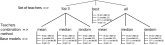
\includegraphics[width=0.9\linewidth]{img/schema}
	\caption{Schema representing the set of experiments conducted in this study.}
	\label{fig:schema}
\end{figure}

		
	We have repeated each experiment 5 times to add more robustness to our results, totaling to 140 training processes. The students initial weights have always been fixed to the pretrained weights for the \textit{ImageNet} classification task, across all the experiments. During training, no layers have been frozen, allowing the optimizer to fine-tune all the weights in the student network. The last layer has been warmed in all the cases to match the normalized soft-targets distribution, as described in section \ref{sec:teachers_comb}.  Each model has been trained for 100 epochs with \textit{Adam} optimizer \cite{Kingma14} and a learning rate of $10^{-6}$.
	
	 In our experiments we fix $S=0.35$ and determine the value of $T$ for every pretrained model using the bisection method with the transfer data set. The value of S has been chosen so that it produces an average temperature across the models of 2.0, which is close to the range recommended in \cite{hinton2015}. We tried doubling the temperature parameter concluding that there were no noticeable improvements.
	 
	 To run the experiments, we used a single \textit{Nvidia RTX 2080ti} GPU, and the code has been implemented in \textit{Tensorflow 2.0}. The repository of code is public and can be found in the following URL: \url{https://github.com/ivallesp/cocktailnet}
		
	\subsection{Results}  \label{sec:results}
	Tables \ref{tab:results1} and \ref{tab:results5} shows the results achieved by each of the models trained. The results are expressed as the average metric $\pm$ the standard ertror. As it can be seen in the table, the proposed methodology is able to increase the accuracy of the models up to +X.X\%, +X.X\%, +X.X\% and +X.X\% for the \textit{MobileNetV2}, \textit{EfficientNetB0}, \textit{DenseNet} and \textit{Xception} students, respectively. In general, the best combination method has been XXXXX although in the case of \textit{DenseNet} it YYYYYY showed better results. 
	
	\begin{table}[h]
	\small
	\centering

	\caption{Results in top-1 accuracy (\%) for all the experiments. Each column in the table represents a different teacher set}
	\begin{tabular}{rrrrrr}\toprule
		& &Baseline &Best &Top3 &All \\
		Student, &Comb. method & & & & \\\midrule
		MobileNetV2 &Mean &72.98 &$\mu \pm \sigma$ &$\mu \pm \sigma$ &$\mu \pm \sigma$ \\
		&Median &72.98 &- &$\mu \pm \sigma$ &$\mu \pm \sigma$ \\
		&Random &72.98 &- &$\mu \pm \sigma$ &$\mu \pm \sigma$ \\
		& & & & & \\
		EfficientNetB0 &Mean &75.17 &$\mu \pm \sigma$ &$\mu \pm \sigma$ &$\mu \pm \sigma$ \\
		&Median &75.17 &- &$\mu \pm \sigma$ &$\mu \pm \sigma$ \\
		&Random &75.17 &- &$\mu \pm \sigma$ &$\mu \pm \sigma$ \\
		& & & & & \\
		DenseNet121 &Mean &75.44 &$\mu \pm \sigma$ &$\mu \pm \sigma$ &$\mu \pm \sigma$ \\
		&Median &75.44 &- &$\mu \pm \sigma$ &$\mu \pm \sigma$ \\
		&Random &75.44 &- &$\mu \pm \sigma$ &$\mu \pm \sigma$ \\
		& & & & & \\
		Xception &Mean &78.92 &$\mu \pm \sigma$ &$\mu \pm \sigma$ &$\mu \pm \sigma$ \\
		&Median &78.92 &- &$\mu \pm \sigma$ &$\mu \pm \sigma$ \\
		&Random &78.92 &- &$\mu \pm \sigma$ &$\mu \pm \sigma$ \\
		\bottomrule
	\end{tabular}
	\label{tab:results1}
	\end{table}

	\begin{table}[h]
	\small
	\centering

	\caption{Results in top-5 accuracy (\%) for all the experiments. Each column in the table represents a different teacher set}
	\begin{tabular}{rrrrrr}\toprule
		& &Baseline &Best &Top3 &All \\
		Student, &Comb. method & & & & \\\midrule
		MobileNetV2 &Mean &XXX &$\mu \pm \sigma$ &$\mu \pm \sigma$ &$\mu \pm \sigma$ \\
		&Median &XXX &- &$\mu \pm \sigma$ &$\mu \pm \sigma$ \\
		&Random &XXX &- &$\mu \pm \sigma$ &$\mu \pm \sigma$ \\
		& & & & & \\
		EfficientNetB0 &Mean &XXX &$\mu \pm \sigma$ &$\mu \pm \sigma$ &$\mu \pm \sigma$ \\
		&Median &XXX&- &$\mu \pm \sigma$ &$\mu \pm \sigma$ \\
		&Random &XXX&- &$\mu \pm \sigma$ &$\mu \pm \sigma$ \\
		& & & & & \\
		DenseNet121 &Mean &XXX &$\mu \pm \sigma$ &$\mu \pm \sigma$ &$\mu \pm \sigma$ \\
		&Median &XXX &- &$\mu \pm \sigma$ &$\mu \pm \sigma$ \\
		&Random &XXX &- &$\mu \pm \sigma$ &$\mu \pm \sigma$ \\
		& & & & & \\
		Xception &Mean &XXX &$\mu \pm \sigma$ &$\mu \pm \sigma$ &$\mu \pm \sigma$ \\
		&Median &XXX &- &$\mu \pm \sigma$ &$\mu \pm \sigma$ \\
		&Random &XXX &- &$\mu \pm \sigma$ &$\mu \pm \sigma$ \\
		\bottomrule
	\end{tabular}
	\label{tab:results5}
\end{table}
	
	Figures XX and YY show the training curves for all the cases. As it can be seen although we reported the accuracy of the 100th epoch, there are cases where earlier epochs showed a slightly better performance.
	
	In our experiments, we noticed that choosing a very small learning rate was crucial to achieve the performance reported. Higher learning rates ( $10^{-5}$ and  $10^{-3}$) were tested leading to worse performances (sometimes even worse than the original pretrained model). We hypothesize that this effect is due to catastrophic forgetting, which leads to overfitting to the transfer set when the learning rate is too big.
			
	\section{Conclusions}  \label{sec:conclusions}
	We have shown how by using simple knowledge distillation techniques it is possible to increase the accuracy of the smallest pretrained models in just few training epochs. In our opinion, this opens potential new research lines towards more sophisticated teacher blending techniques or distillation methodologies. This can also motivate the research of novel training techniques, alternative or complementary to \textit{backpropagation}, as it seems that the pretrained models still didn't reach their maximum capacity.
	
	
	\section{Acknowledgements}
	We would like to thank \textit{David Vallés-Pérez} for his helpful feedback and fruitful discussion.
	\newpage
	
	\bibliographystyle{abbrvnat}
	\bibliography{mybib}
	
	% Catastrophic forgetting is usually not a problem in pretrained learning because the target task is different than the original task. It is not the case here. 
	% Incremental training: parameters of model i are used as initialization for parameters of model i+1
\end{document}